\documentclass[aspectratio=169]{beamer}

\usetheme{default}
\usecolortheme{dove}

\setbeamertemplate{navigation symbols}{}
\setbeamertemplate{footline}{%
  \hfill\insertframenumber\,/\,\inserttotalframenumber\hspace{0.5em}\vspace{0.5em}%
}

\definecolor{popblue}{RGB}{52, 101, 164}
\definecolor{sampred}{RGB}{204, 0, 0}
\definecolor{paramgreen}{RGB}{0, 140, 70}
\definecolor{warnred}{RGB}{180, 40, 40}
\definecolor{orange1}{RGB}{220, 120, 0}

\setbeamercolor{frametitle}{fg=popblue}
\setbeamercolor{title}{fg=popblue}

\usepackage{pgfplots}
\usepackage{tikz}
\usetikzlibrary{shapes, arrows.meta, positioning, calc, decorations.pathreplacing, patterns}
\pgfplotsset{compat=1.18}
\usepackage{amsmath, amssymb}

\title{Lecture 2a: Point Estimation}
\subtitle{Method of Moments and Maximum Likelihood}
\date{}

\begin{document}

% ============================================================
\begin{frame}
\titlepage
\end{frame}

% ============================================================
\begin{frame}
\frametitle{The Estimation Problem}
\begin{center}
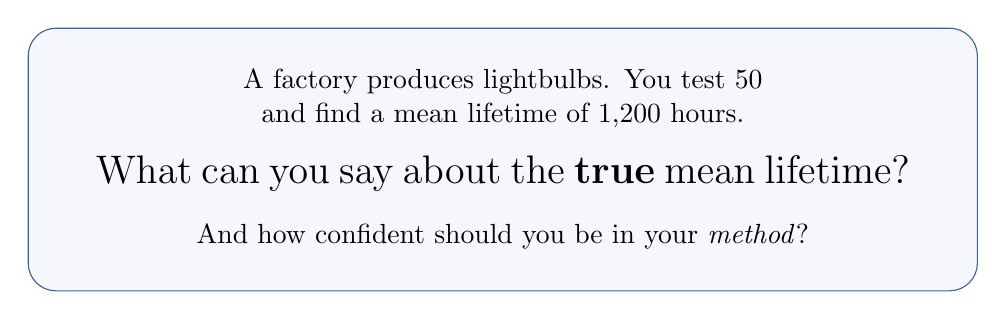
\begin{tikzpicture}
  \node[draw=popblue, fill=popblue!5, rounded corners=10pt, text width=11cm, align=center, inner sep=15pt] {
    A factory produces lightbulbs. You test 50 and find a mean lifetime of 1{,}200 hours.\\[10pt]
    {\Large What can you say about the \textbf{true} mean lifetime?}\\[10pt]
    And how confident should you be in your \textit{method}?
  };
\end{tikzpicture}
\end{center}
\end{frame}

\begin{frame}
\frametitle{From Data to Parameters}
\begin{center}
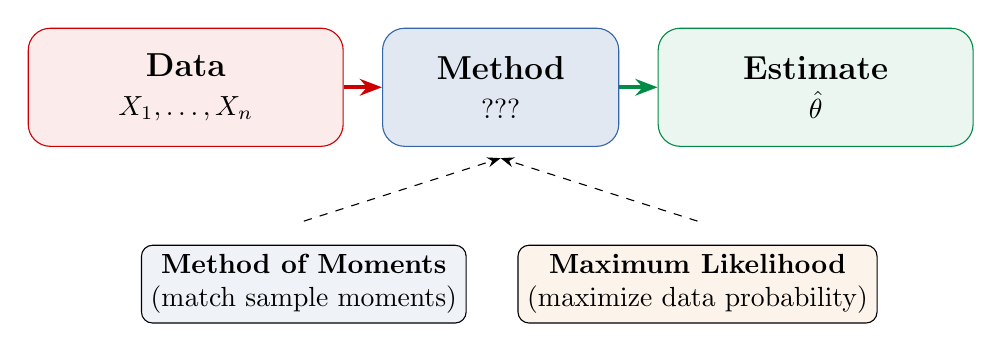
\begin{tikzpicture}[
  arrow/.style={-{Stealth[length=8pt]}, line width=1.5pt}
]
  % Data
  \node[draw=sampred, fill=sampred!8, rounded corners=8pt, minimum width=4cm, minimum height=1.5cm, font=\large\bfseries, align=center] (data) at (-4, 0) {Data\\{\normalsize\normalfont $X_1, \ldots, X_n$}};

  % Black box
  \node[draw=popblue, fill=popblue!15, rounded corners=8pt, minimum width=3cm, minimum height=1.5cm, font=\large\bfseries, align=center] (method) at (0, 0) {Method\\{\normalsize\normalfont ???}};

  % Estimate
  \node[draw=paramgreen, fill=paramgreen!8, rounded corners=8pt, minimum width=4cm, minimum height=1.5cm, font=\large\bfseries, align=center] (est) at (4, 0) {Estimate\\{\normalsize\normalfont $\hat{\theta}$}};

  \draw[arrow, sampred] (data) -- (method);
  \draw[arrow, paramgreen] (method) -- (est);

  % Two methods below
  \node[draw, rounded corners=4pt, fill=popblue!8, minimum width=4cm, font=\normalsize, align=center] at (-2.5, -2.5) {\textbf{Method of Moments}\\(match sample moments)};
  \node[draw, rounded corners=4pt, fill=orange1!8, minimum width=4cm, font=\normalsize, align=center] at (2.5, -2.5) {\textbf{Maximum Likelihood}\\(maximize data probability)};

  \draw[-{Stealth}, dashed] (-2.5, -1.7) -- (0, -0.9);
  \draw[-{Stealth}, dashed] (2.5, -1.7) -- (0, -0.9);
\end{tikzpicture}
\end{center}
\end{frame}

% ============================================================
\section{Method of Moments}

\begin{frame}
\frametitle{Method of Moments (MoM)}

\textbf{Idea:} Set population moments equal to sample moments, then solve for the parameters.

\vspace{0.4cm}
\begin{center}
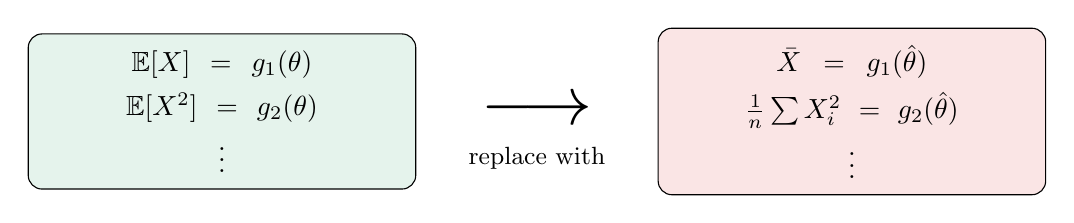
\begin{tikzpicture}[
  mombox/.style={draw, rounded corners=5pt, minimum height=1cm, text width=4.5cm, align=center, font=\normalsize, inner sep=6pt}
]
  \node[mombox, fill=paramgreen!10] at (-4, 0) {
    $\mathbb{E}[X] = g_1(\theta)$\\[4pt]
    $\mathbb{E}[X^2] = g_2(\theta)$\\[2pt]
    $\vdots$
  };

  \node[font=\Huge] at (0, 0) {$\longrightarrow$};
  \node[font=\small] at (0, -0.6) {replace with};

  \node[mombox, fill=sampred!10] at (4, 0) {
    $\bar{X} = g_1(\hat{\theta})$\\[4pt]
    $\frac{1}{n}\sum X_i^2 = g_2(\hat{\theta})$\\[2pt]
    $\vdots$
  };
\end{tikzpicture}
\end{center}

\vspace{0.5cm}
\begin{columns}
\begin{column}{0.48\textwidth}
  \textcolor{paramgreen}{\textbf{Pros:}}
  \begin{itemize}\small
    \item Simple, quick to compute
    \item No distributional assumption needed for computation
  \end{itemize}
\end{column}
\begin{column}{0.48\textwidth}
  \textcolor{warnred}{\textbf{Cons:}}
  \begin{itemize}\small
    \item Can give impossible values (e.g., $\hat{\sigma}^2 < 0$)
    \item Generally less efficient than MLE
    \item Awkward with many parameters
  \end{itemize}
\end{column}
\end{columns}
\end{frame}

\begin{frame}
\frametitle{MoM Example: Normal Distribution}
\begin{center}
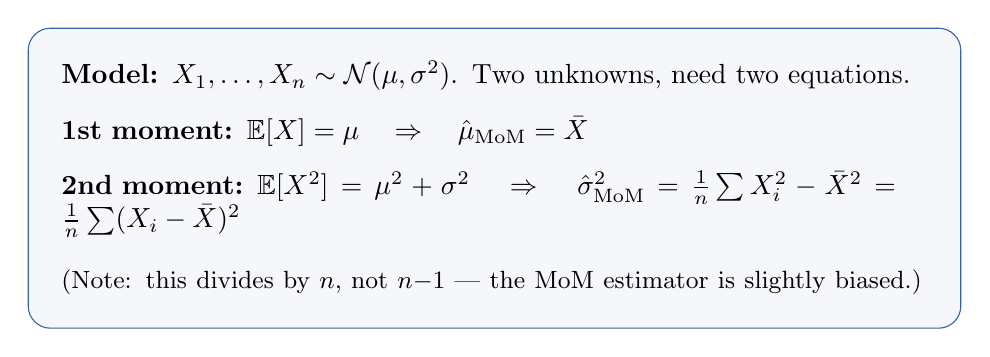
\begin{tikzpicture}
  \node[draw=popblue, fill=popblue!5, rounded corners=8pt, text width=11cm, align=left, inner sep=12pt] {
    \textbf{Model:} $X_1, \ldots, X_n \sim \mathcal{N}(\mu, \sigma^2)$. Two unknowns, need two equations.\\[8pt]
    \textbf{1st moment:} $\mathbb{E}[X] = \mu \quad\Rightarrow\quad \hat{\mu}_{\text{MoM}} = \bar{X}$\\[8pt]
    \textbf{2nd moment:} $\mathbb{E}[X^2] = \mu^2 + \sigma^2 \quad\Rightarrow\quad \hat{\sigma}^2_{\text{MoM}} = \frac{1}{n}\sum X_i^2 - \bar{X}^2 = \frac{1}{n}\sum(X_i - \bar{X})^2$\\[10pt]
    \small (Note: this divides by $n$, not $n{-}1$ --- the MoM estimator is slightly biased.)
  };
\end{tikzpicture}
\end{center}
\end{frame}

% ============================================================
\section{Likelihood}

\begin{frame}
\frametitle{The Likelihood Function}

\begin{center}
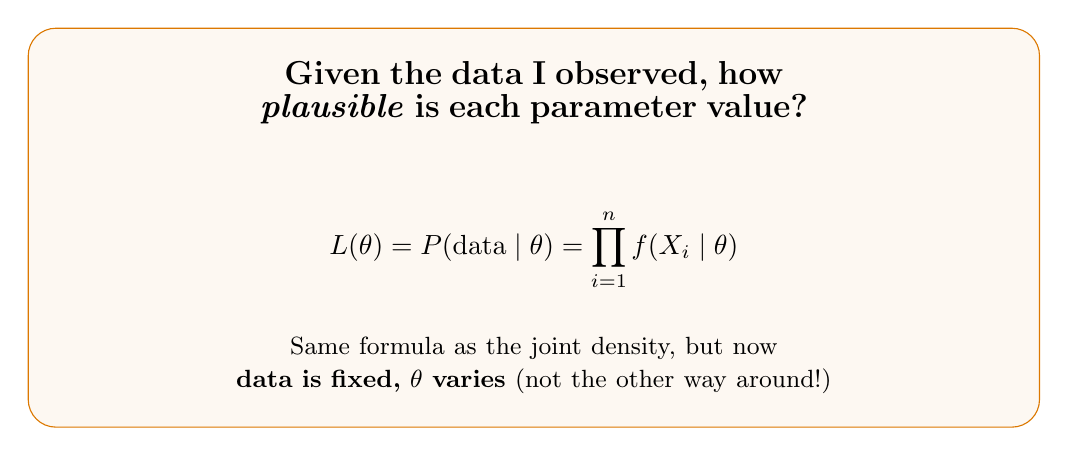
\begin{tikzpicture}
  % Big idea box
  \node[draw=orange1, fill=orange1!5, rounded corners=10pt, text width=12cm, align=center, inner sep=12pt] {
    {\large\bfseries Given the data I observed, how \textit{plausible} is each parameter value?}\\[10pt]
    $$L(\theta) = P(\text{data} \mid \theta) = \prod_{i=1}^n f(X_i \mid \theta)$$\\[6pt]
    \small Same formula as the joint density, but now\\
    \textbf{data is fixed, $\theta$ varies} (not the other way around!)
  };
\end{tikzpicture}
\end{center}
\end{frame}

\begin{frame}
\frametitle{Likelihood: Coin Flip Example}
\begin{center}
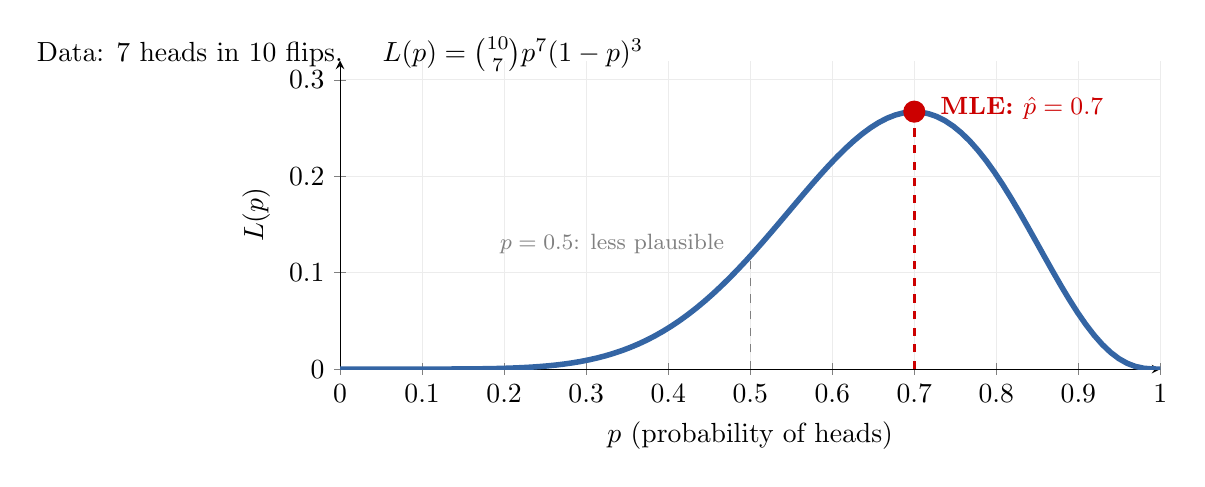
\begin{tikzpicture}
  \node[font=\normalsize] at (0, 4) {Data: 7 heads in 10 flips. \quad $L(p) = \binom{10}{7} p^7 (1-p)^3$};

  \begin{axis}[
    width=12cm, height=5.5cm,
    xlabel={$p$ (probability of heads)},
    ylabel={$L(p)$},
    xmin=0, xmax=1,
    ymin=0, ymax=0.32,
    axis lines=left,
    grid=major, grid style={gray!15},
    every axis plot/.append style={line width=2pt, samples=100}
  ]
    \addplot[popblue, domain=0:1] {120 * x^7 * (1-x)^3};

    % MLE marker
    \draw[very thick, sampred, dashed] (axis cs:0.7, 0) -- (axis cs:0.7, 0.267);
    \fill[sampred] (axis cs:0.7, 0.267) circle (4pt);
    \node[font=\small\bfseries, sampred, right] at (axis cs:0.72, 0.27) {MLE: $\hat{p} = 0.7$};

    % Other values
    \draw[thin, dashed, gray] (axis cs:0.5, 0) -- (axis cs:0.5, 0.117);
    \node[font=\footnotesize, gray, left] at (axis cs:0.48, 0.13) {$p=0.5$: less plausible};
  \end{axis}
\end{tikzpicture}
\end{center}
\end{frame}

\begin{frame}
\frametitle{Log-Likelihood: Why We Prefer It}
\begin{center}
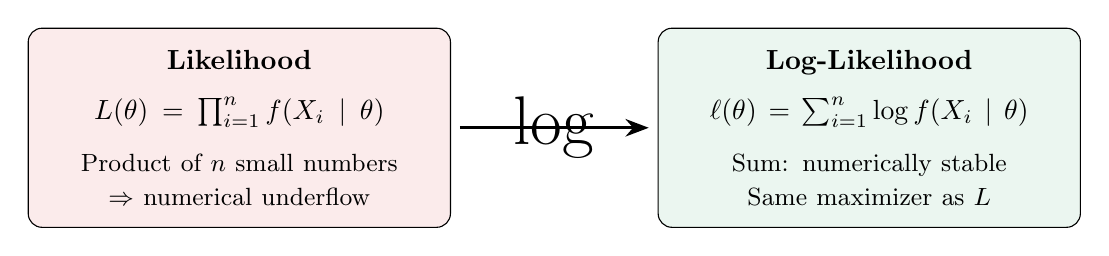
\begin{tikzpicture}[
  llbox/.style={draw, rounded corners=5pt, minimum height=2.5cm, text width=4.8cm, align=center, inner sep=8pt}
]
  \node[llbox, fill=sampred!8] at (-4, 0) {
    \textbf{Likelihood}\\[6pt]
    $L(\theta) = \prod_{i=1}^n f(X_i \mid \theta)$\\[8pt]
    \small Product of $n$ small numbers\\
    $\Rightarrow$ numerical underflow
  };

  \node[font=\Huge] at (0, 0) {$\log$};
  \draw[-{Stealth}, very thick] (-1.2, 0) -- (1.2, 0);

  \node[llbox, fill=paramgreen!8] at (4, 0) {
    \textbf{Log-Likelihood}\\[6pt]
    $\ell(\theta) = \sum_{i=1}^n \log f(X_i \mid \theta)$\\[8pt]
    \small Sum: numerically stable\\
    Same maximizer as $L$
  };
\end{tikzpicture}
\end{center}

\vspace{0.5cm}
\textbf{Score function:} $s(\theta) = \frac{\partial \ell(\theta)}{\partial \theta}$ \quad --- the gradient of the log-likelihood.\\[4pt]
\small At the MLE: $s(\hat{\theta}) = 0$ \quad (first-order condition).
\end{frame}

% ============================================================
\section{Maximum Likelihood Estimation}

\begin{frame}
\frametitle{Maximum Likelihood Estimation}

\begin{center}
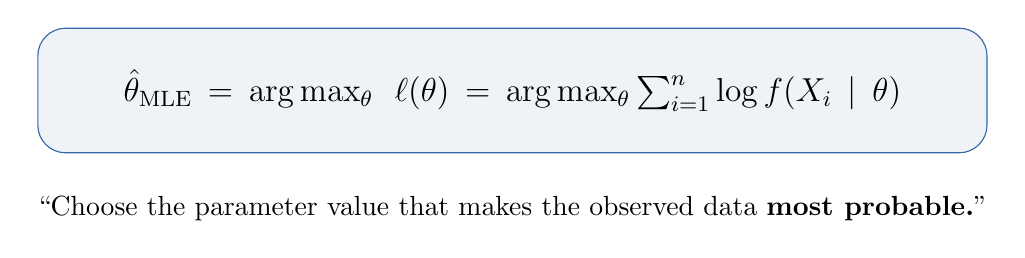
\begin{tikzpicture}
  \node[draw=popblue, fill=popblue!8, rounded corners=10pt, text width=11cm, align=center, inner sep=15pt, font=\large] {
    $\hat{\theta}_{\text{MLE}} = \arg\max_\theta \; \ell(\theta) = \arg\max_\theta \sum_{i=1}^n \log f(X_i \mid \theta)$
  };
  \node[font=\normalsize] at (0, -1.5) {``Choose the parameter value that makes the observed data \textbf{most probable.}''};
\end{tikzpicture}
\end{center}

\vspace{0.3cm}
\textbf{Recipe:}
\begin{enumerate}
  \item Write down the log-likelihood $\ell(\theta)$
  \item Take the derivative and set $\frac{\partial \ell}{\partial \theta} = 0$
  \item Solve for $\hat{\theta}$
  \item Check second-order condition ($\frac{\partial^2 \ell}{\partial \theta^2} < 0$)
\end{enumerate}
\end{frame}

\begin{frame}
\frametitle{MLE: Bernoulli (Coin Fairness)}
\begin{center}
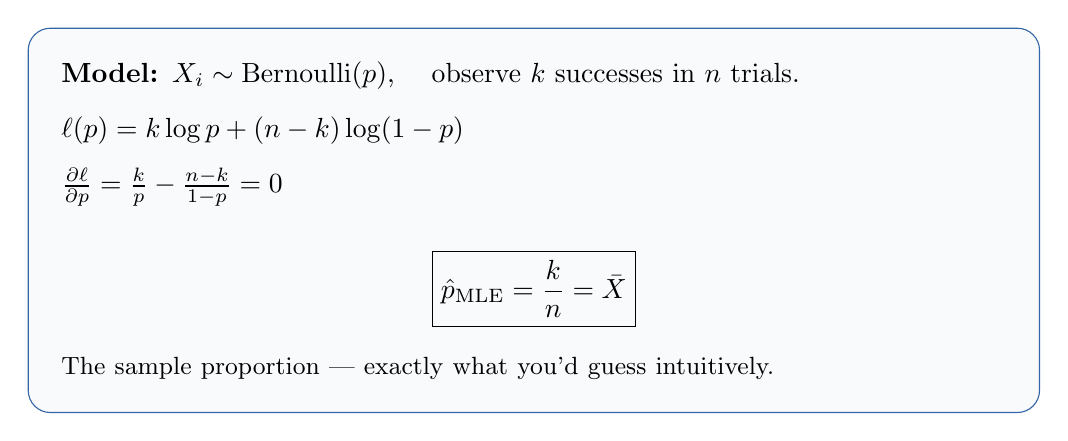
\begin{tikzpicture}
  \node[draw=popblue, fill=popblue!3, rounded corners=8pt, text width=12cm, align=left, inner sep=12pt] {
    \textbf{Model:} $X_i \sim \text{Bernoulli}(p)$, \quad observe $k$ successes in $n$ trials.\\[8pt]
    $\ell(p) = k\log p + (n-k)\log(1-p)$\\[8pt]
    $\frac{\partial\ell}{\partial p} = \frac{k}{p} - \frac{n-k}{1-p} = 0$\\[8pt]
    $$\boxed{\hat{p}_{\text{MLE}} = \frac{k}{n} = \bar{X}}$$\\[4pt]
    \small The sample proportion --- exactly what you'd guess intuitively.
  };
\end{tikzpicture}
\end{center}
\end{frame}

\begin{frame}
\frametitle{MLE: Normal (Measurement Error)}
\begin{center}
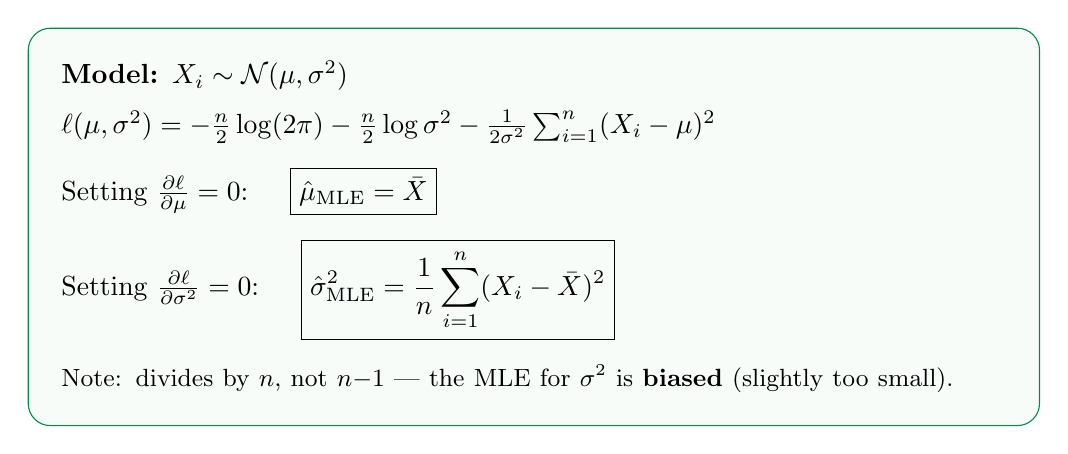
\begin{tikzpicture}
  \node[draw=paramgreen, fill=paramgreen!3, rounded corners=8pt, text width=12cm, align=left, inner sep=12pt] {
    \textbf{Model:} $X_i \sim \mathcal{N}(\mu, \sigma^2)$\\[6pt]
    $\ell(\mu, \sigma^2) = -\frac{n}{2}\log(2\pi) - \frac{n}{2}\log\sigma^2 - \frac{1}{2\sigma^2}\sum_{i=1}^n(X_i - \mu)^2$\\[8pt]
    Setting $\frac{\partial\ell}{\partial\mu} = 0$: \quad $\boxed{\hat{\mu}_{\text{MLE}} = \bar{X}}$\\[8pt]
    Setting $\frac{\partial\ell}{\partial\sigma^2} = 0$: \quad $\boxed{\hat{\sigma}^2_{\text{MLE}} = \frac{1}{n}\sum_{i=1}^n(X_i - \bar{X})^2}$\\[8pt]
    \small Note: divides by $n$, not $n{-}1$ --- the MLE for $\sigma^2$ is \textbf{biased} (slightly too small).
  };
\end{tikzpicture}
\end{center}
\end{frame}

\begin{frame}
\frametitle{MLE: Poisson (Rare Events)}
\begin{center}
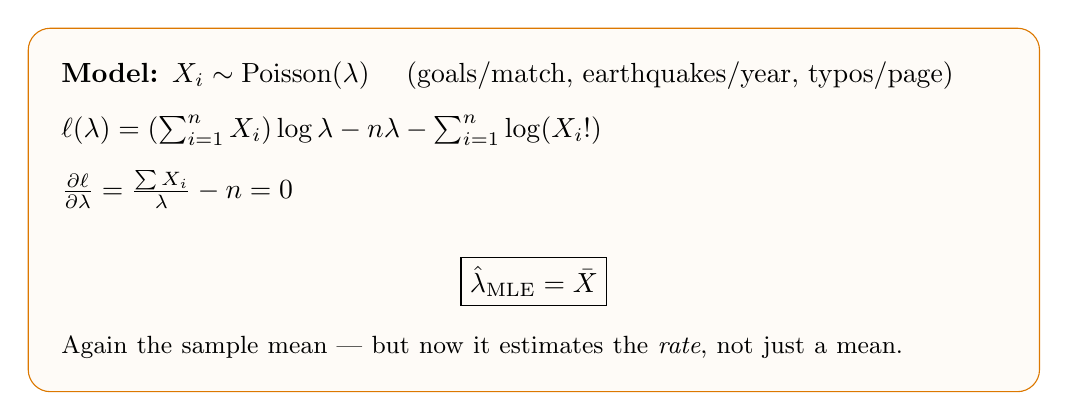
\begin{tikzpicture}
  \node[draw=orange1, fill=orange1!3, rounded corners=8pt, text width=12cm, align=left, inner sep=12pt] {
    \textbf{Model:} $X_i \sim \text{Poisson}(\lambda)$ \quad (goals/match, earthquakes/year, typos/page)\\[8pt]
    $\ell(\lambda) = \left(\sum_{i=1}^n X_i\right)\log\lambda - n\lambda - \sum_{i=1}^n\log(X_i!)$\\[8pt]
    $\frac{\partial\ell}{\partial\lambda} = \frac{\sum X_i}{\lambda} - n = 0$\\[8pt]
    $$\boxed{\hat{\lambda}_{\text{MLE}} = \bar{X}}$$\\[4pt]
    \small Again the sample mean --- but now it estimates the \textit{rate}, not just a mean.
  };
\end{tikzpicture}
\end{center}
\end{frame}

\begin{frame}
\frametitle{MLE: Exponential (Waiting Times)}
\begin{center}
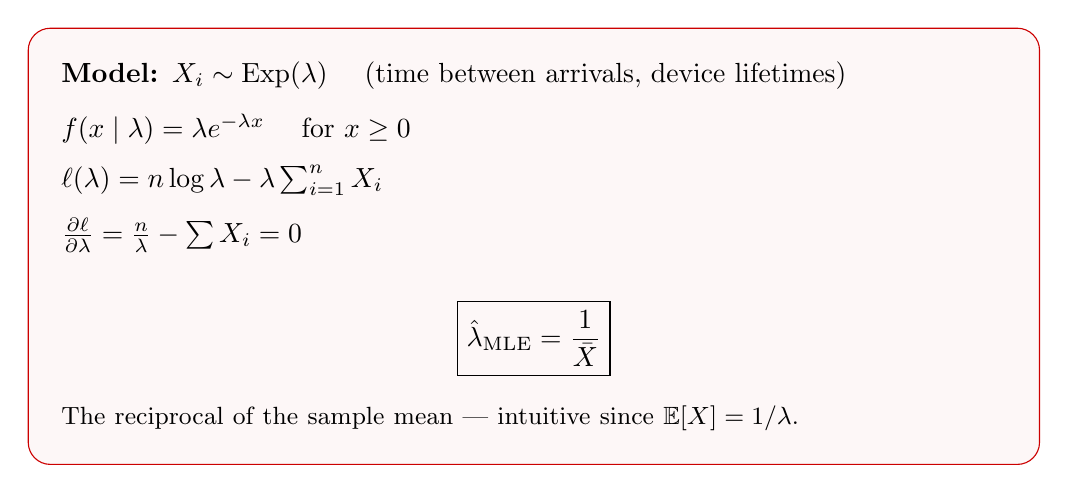
\begin{tikzpicture}
  \node[draw=sampred, fill=sampred!3, rounded corners=8pt, text width=12cm, align=left, inner sep=12pt] {
    \textbf{Model:} $X_i \sim \text{Exp}(\lambda)$ \quad (time between arrivals, device lifetimes)\\[8pt]
    $f(x \mid \lambda) = \lambda e^{-\lambda x}$ \quad for $x \ge 0$\\[6pt]
    $\ell(\lambda) = n\log\lambda - \lambda\sum_{i=1}^n X_i$\\[8pt]
    $\frac{\partial\ell}{\partial\lambda} = \frac{n}{\lambda} - \sum X_i = 0$\\[8pt]
    $$\boxed{\hat{\lambda}_{\text{MLE}} = \frac{1}{\bar{X}}}$$\\[4pt]
    \small The reciprocal of the sample mean --- intuitive since $\mathbb{E}[X] = 1/\lambda$.
  };
\end{tikzpicture}
\end{center}
\end{frame}

\begin{frame}
\frametitle{MLE: Summary of Examples}
\begin{center}
\renewcommand{\arraystretch}{1.8}
\begin{tabular}{lccc}
  \textbf{Distribution} & \textbf{Parameter} & \textbf{MLE} & \textbf{Real-world use} \\
  \hline
  Bernoulli$(p)$ & $p$ & $\bar{X}$ & Coin fairness, conversion rates \\
  Normal$(\mu, \sigma^2)$ & $\mu, \sigma^2$ & $\bar{X}, \;\frac{1}{n}\sum(X_i-\bar{X})^2$ & Measurement error \\
  Poisson$(\lambda)$ & $\lambda$ & $\bar{X}$ & Count data, rare events \\
  Exponential$(\lambda)$ & $\lambda$ & $1/\bar{X}$ & Waiting times, lifetimes \\
  \hline
\end{tabular}
\end{center}

\vspace{0.3cm}
\small All connect to distributions from Module 19.
\end{frame}

% ============================================================
\section{MLE Properties}

\begin{frame}
\frametitle{Invariance Property}
\begin{center}
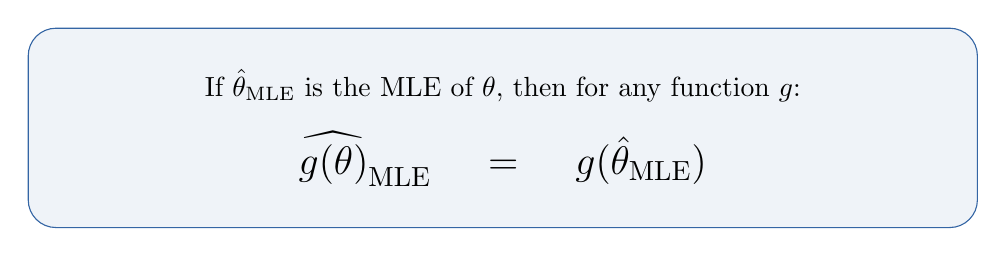
\begin{tikzpicture}
  \node[draw=popblue, fill=popblue!8, rounded corners=10pt, text width=11cm, align=center, inner sep=15pt] {
    If $\hat{\theta}_{\text{MLE}}$ is the MLE of $\theta$, then for any function $g$:\\[10pt]
    {\Large $\widehat{g(\theta)}_{\text{MLE}} = g(\hat{\theta}_{\text{MLE}})$}
  };
\end{tikzpicture}
\end{center}

\vspace{0.5cm}
\textbf{Example:}
\begin{itemize}
  \item MLE of $\lambda$ for Exponential is $\hat{\lambda} = 1/\bar{X}$
  \item Want the MLE of the \textit{mean} $\mu = 1/\lambda$? Just apply $g(\lambda) = 1/\lambda$:
  \item $\hat{\mu}_{\text{MLE}} = 1/\hat{\lambda} = \bar{X}$ \checkmark
\end{itemize}

\vspace{0.3cm}
\small This doesn't hold for method of moments or other estimators in general.
\end{frame}

\begin{frame}
\frametitle{Identifiability}
\begin{center}
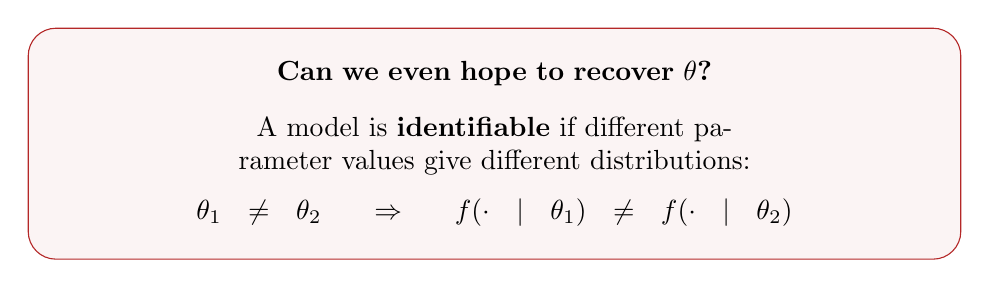
\begin{tikzpicture}
  \node[draw=warnred, fill=warnred!5, rounded corners=10pt, text width=11cm, align=center, inner sep=12pt] {
    \textbf{Can we even hope to recover $\theta$?}\\[8pt]
    A model is \textbf{identifiable} if different parameter values give different distributions:\\[6pt]
    $\theta_1 \ne \theta_2 \;\Rightarrow\; f(\cdot \mid \theta_1) \ne f(\cdot \mid \theta_2)$
  };
\end{tikzpicture}
\end{center}

\vspace{0.4cm}
\textbf{When it fails:}
\begin{itemize}
  \item \textbf{Mixture models:} swapping component labels gives the same distribution
  \item \textbf{Overparameterized models:} more parameters than the data can distinguish
  \item \textbf{Symmetric likelihoods:} multiple maxima, MLE is not unique
\end{itemize}

\vspace{0.3cm}
\small If the model isn't identifiable, no amount of data will help.
\end{frame}

\begin{frame}
\frametitle{Visualizing Non-Identifiability}
\begin{center}
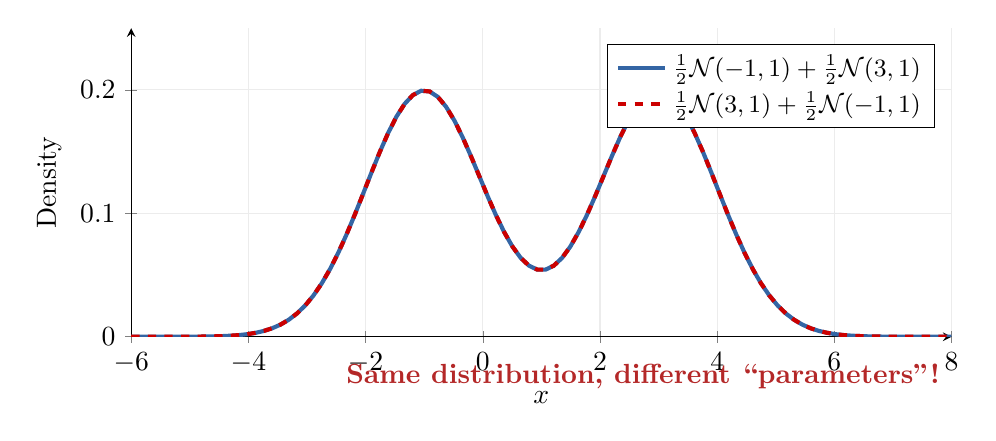
\begin{tikzpicture}
  \begin{axis}[
    width=12cm, height=5.5cm,
    xlabel={$x$},
    ylabel={Density},
    xmin=-6, xmax=8,
    ymin=0, ymax=0.25,
    axis lines=left,
    grid=major, grid style={gray!15},
    every axis plot/.append style={line width=1.5pt, samples=100},
    legend style={at={(0.98,0.95)}, anchor=north east, font=\small}
  ]
    % Same mixture, two parameterizations
    \addplot[popblue, domain=-6:8] {0.5 * exp(-(x+1)^2/2)/sqrt(2*pi) + 0.5 * exp(-(x-3)^2/2)/sqrt(2*pi)};
    \addlegendentry{$\frac{1}{2}\mathcal{N}(-1,1) + \frac{1}{2}\mathcal{N}(3,1)$}

    \addplot[sampred, dashed, domain=-6:8] {0.5 * exp(-(x-3)^2/2)/sqrt(2*pi) + 0.5 * exp(-(x+1)^2/2)/sqrt(2*pi)};
    \addlegendentry{$\frac{1}{2}\mathcal{N}(3,1) + \frac{1}{2}\mathcal{N}(-1,1)$}
  \end{axis}

  \node[font=\normalsize\bfseries, text=warnred] at (6.5, -0.5) {Same distribution, different ``parameters''!};
\end{tikzpicture}
\end{center}
\end{frame}

% ============================================================
\section{Practical}

\begin{frame}
\frametitle{Practical: Implement MLE}
\begin{center}
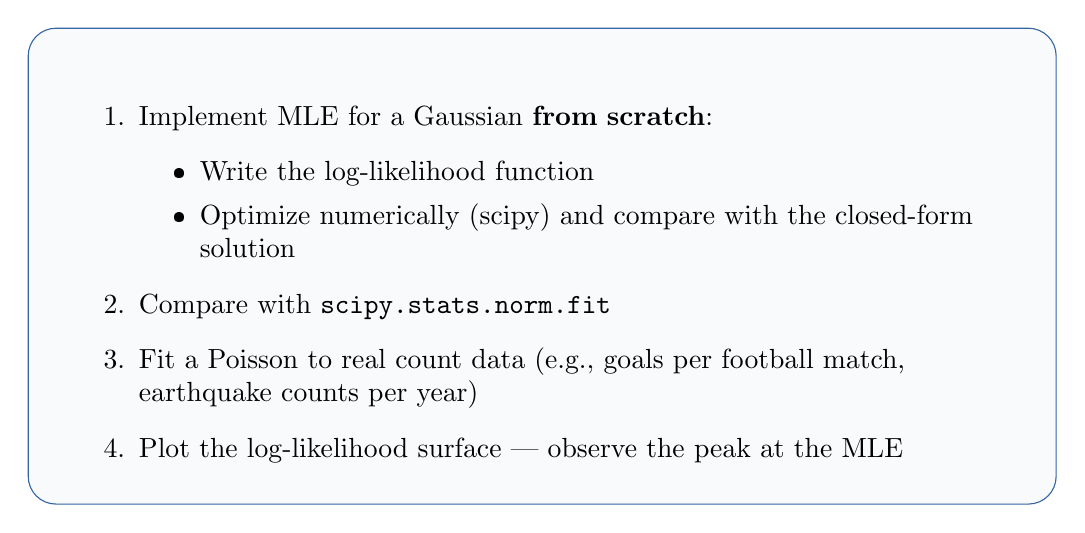
\begin{tikzpicture}
  \node[draw=popblue, fill=popblue!3, rounded corners=10pt, text width=12cm, align=left, inner sep=15pt] {
    \begin{enumerate}
      \item Implement MLE for a Gaussian \textbf{from scratch}:
        \begin{itemize}
          \item Write the log-likelihood function
          \item Optimize numerically (scipy) and compare with the closed-form solution
        \end{itemize}
      \item Compare with \texttt{scipy.stats.norm.fit}
      \item Fit a Poisson to real count data (e.g., goals per football match, earthquake counts per year)
      \item Plot the log-likelihood surface --- observe the peak at the MLE
    \end{enumerate}
  };
\end{tikzpicture}
\end{center}
\end{frame}

\begin{frame}
\begin{center}
  {\Huge\bfseries\textcolor{popblue}{Questions?}}

  \vspace{1cm}

  {\large Next lecture: MAP, Priors, and the Bayesian Perspective}
\end{center}
\end{frame}

\end{document}
